\documentclass[11pt]{beamer}
\usetheme{Boadilla}
\usepackage[utf8]{inputenc}
\usepackage{amsmath}
\usepackage{amsfonts}
\usepackage{amssymb}

\author{Hermilo Cortés González}
\title{Taller Ecología del Movimiento}
%\setbeamercovered{transparent} 
%\setbeamertemplate{navigation symbols}{} 
%\logo{} 
%\institute{} 
\date{\today} 
%\subject{} 
\begin{document}

\begin{frame}
\titlepage
\end{frame}

%\begin{frame}
%\tableofcontents
%\end{frame}

\begin{frame}{¿En qué lugar pasas tu día en Ciencias?}
	\begin{figure}
		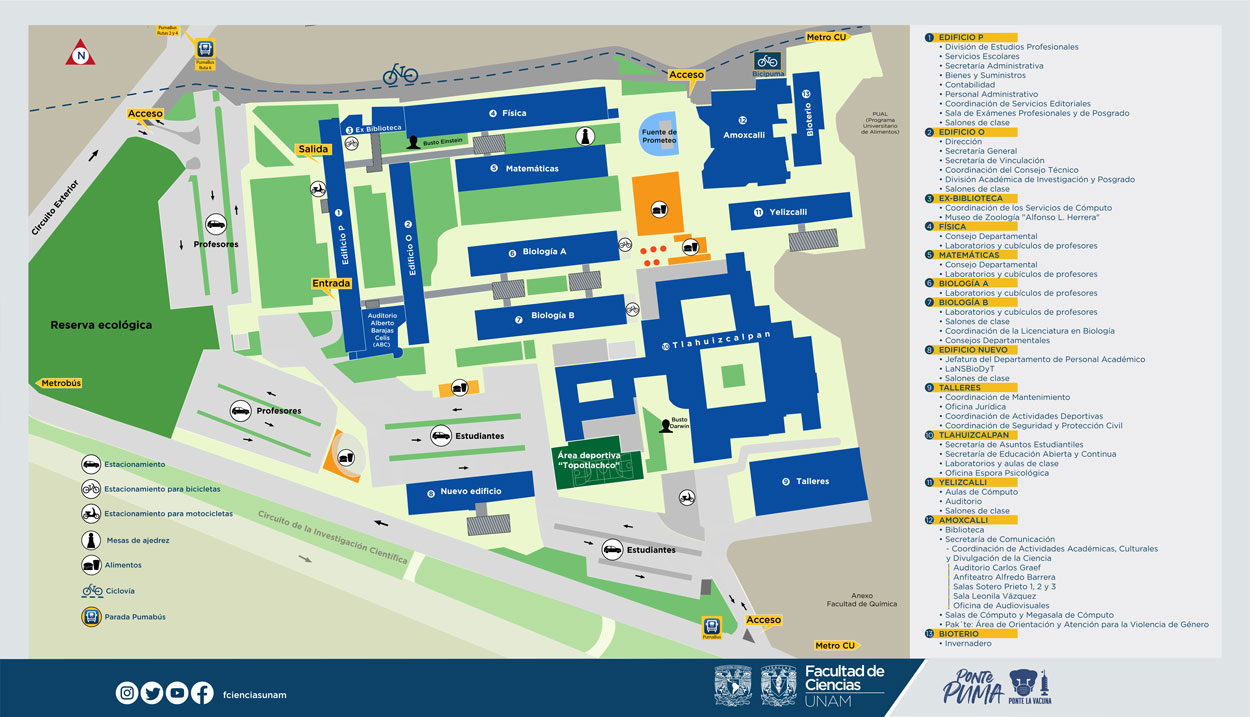
\includegraphics[scale=0.28]{images/MAPA_Fac_2021.jpg}
	\end{figure}
\end{frame}


\begin{frame}{Marco conceptual de la Ecología del Movimiento \cite{nathan2008movement}}

El marco incorpora dos grandes componentes: 
	\begin{itemize}
		\item Componente basado en el individuo.
		\item Componente basado en los factores externos que influyen en las causas, mecanismos y patrones de movimiento.
	\end{itemize}


\end{frame}

\begin{frame}{Componente basado en el individuo}
Preguntas

	\begin{enumerate}
		\item ¿Por qué se mueven?
		\item ¿Dónde se mueven?
		\item ¿Cómo se mueven?			
	\end{enumerate}	

Proceso de toma de decisión de movimiento del individuo :			
				\begin{center}
					 \textbf{¿Cómo se le asigna una importancia relativa al comportamiento de acuerdo a diferentes objetivos como reproducción, alimentación, descanso, etc?¿Cómo entendemos el movimiento de acuerdo a distintas metas o propositos?}
				\end{center}
\end{frame}

\begin{frame}{Componente basado en los factores externos}
	\begin{itemize}
		\item ¿Cómo está cambiando el entorno-contexto donde se desarrolla el individuo?
	\end{itemize}
\end{frame}

\begin{frame}{Tipología de movimiento}

Los principales tipos de movimiento son los de:
	
	\begin{enumerate}
		\item \textbf{Residencia o área de actividad estable} son los movimientos registrados en áreas bien definidas y estables para distintos años. 
		\item \textbf{Migración} es el movimiento estacional-periódico estable de largas distancias entre distintas localidades. Corresponden a movimientos de acuerdo a estaciones del año.
		\item \textbf{Dispersión} es el movimiento en el que la población o individuo deja la localidad ocupada y se mueve hacia una localidad diferente. Ambas áreas, la dejada y la de llegada, son ocupadas por periodos largos de tiempo.
		\item \textbf{Nomadismo} movimiento que tiene una frecuencia alta, no estacional o periódica, y tampoco estable tanto en tiempo de permanencia y de dirección.  
	\end{enumerate}
\end{frame}

\begin{frame}{Net squared displacement (NSD)}
Una forma de distinguir estos tipos de movimientos es mediante el \textbf{Net squared displacement (NSD)}. Este indicador mide la distancia a partir de un punto de inicio de la trayectoria, donde inicia el seguimiento, hasta el punto final de seguimiento.

De acuerdo al NSD, en teoría, se espera que el movimiento de migración tenga una forma de U invertida, lo que quiere decir que la población se aleja de la localidad inicial, permanece en una área provisional por un tiempo,y regresa a la localidad inicial, o una área relativamente cercana. La dispersión tendía la forma de una distribución normal acumulada, donde la población vive en una población inicial y se mueve a otra localidad diferente y ya no regresa a la localidad inicial. El movimiento de nomadismo presenta una linea con pendiente positiva donde la población se aleja más y más de donde comenzó el seguimiento. Para la residencia o área de actividad estable, la linea del NSD se espera sea una linea horizontal, o que existan oscilaciones alrededor de esta.
\end{frame}


\begin{frame}{Limpieza de datos de movimiento}
	\begin{itemize}
		\item Ajustar lo datos al sistema de referencia adecuado del área de análisis.

		\item  Remover valores duplicados.

		\item  Ajustar los datos a la zona horaria del área de análisis.

		\item  Generar una ventana periódica, es decir, que las localizaciones estén espaciadas en un segmento determinado (1 hr, 1 día, 1, semana, etc) para trabajar con los datos recolectados

	\end{itemize}
\end{frame}


\begin{frame}{Referencias}
\bibliographystyle{apalike} 
\bibliography{taller_eco_mov.bib}
\end{frame}

\end{document}